
%input{uls.tex} % run paper_uls.py in the scripts directory to update uls.tex
% non-spinning
\def\BNSul{\ensuremath{1.4 \times 10^{-2}}}
\def\NSBHul{\ensuremath{3.6 \times 10^{-3}}}
\def\BBHul{\ensuremath{7.3 \times 10^{-4}}}

% spinning
\def\SNSBHul{\ensuremath{4.4 \times 10^{-3}}}
\def\SBBHul{\ensuremath{9.0 \times 10^{-4}}}

% BNS NUMBERS
%%%%%%%%%%%%%%%%%%%%%%%%%%%%%%%%%%%%%%%
\def\BNStripleCumLum{\ensuremath{490}}
\def\BNSHoneLoneCumLum{\ensuremath{410}}
\def\BNSHtwoLoneCumLum{\ensuremath{110}}

\def\BNStripleCalErr{\ensuremath{23\%}}
\def\BNSHoneLoneCalErr{\ensuremath{23\%}}
\def\BNSHtwoLoneCalErr{\ensuremath{26\%}}

\def\BNStripleMonErr{\ensuremath{3\%}}
\def\BNSHoneLoneMonErr{\ensuremath{7\%}}
\def\BNSHtwoLoneMonErr{\ensuremath{10\%}}

\def\BNStripleWavErr{\ensuremath{31\%}}
\def\BNSHoneLoneWavErr{\ensuremath{32\%}}
\def\BNSHtwoLoneWavErr{\ensuremath{31\%}}

\def\BNStripleGDErr{\ensuremath{16\%}}
\def\BNSHoneLoneGDErr{\ensuremath{16\%}}
\def\BNSHtwoLoneGDErr{\ensuremath{3\%}}

\def\BNStripleGMErr{\ensuremath{19\%}}
\def\BNSHoneLoneGMErr{\ensuremath{19\%}}
\def\BNSHtwoLoneGMErr{\ensuremath{17\%}}
%%%%%%%%%%%%%%%%%%%%%%%%%%%%%%%%%%%%%%%

% BBH NUMBERS
%%%%%%%%%%%%%%%%%%%%%%%%%%%%%%%%%%%%%%%
\def\BBHtripleCumLum{\ensuremath{11000}}
\def\BBHHoneLoneCumLum{\ensuremath{9400}}
\def\BBHHtwoLoneCumLum{\ensuremath{2200}}

\def\BBHtripleCalErr{\ensuremath{25\%}}
\def\BBHHoneLoneCalErr{\ensuremath{24\%}}
\def\BBHHtwoLoneCalErr{\ensuremath{31\%}}

\def\BBHtripleMonErr{\ensuremath{3\%}}
\def\BBHHoneLoneMonErr{\ensuremath{7\%}}
\def\BBHHtwoLoneMonErr{\ensuremath{10\%}}

\def\BBHtripleWavErr{\ensuremath{33\%}}
\def\BBHHoneLoneWavErr{\ensuremath{34\%}}
\def\BBHHtwoLoneWavErr{\ensuremath{38\%}}

\def\BBHtripleGDErr{\ensuremath{13\%}}
\def\BBHHoneLoneGDErr{\ensuremath{15\%}}
\def\BBHHtwoLoneGDErr{\ensuremath{15\%}}

\def\BBHtripleGMErr{\ensuremath{16\%}}
\def\BBHHoneLoneGMErr{\ensuremath{17\%}}
\def\BBHHtwoLoneGMErr{\ensuremath{18\%}}
%%%%%%%%%%%%%%%%%%%%%%%%%%%%%%%%%%%%%%%

% NSBH NUMBERS
%%%%%%%%%%%%%%%%%%%%%%%%%%%%%%%%%%%%%%%
\def\NSBHtripleCumLum{\ensuremath{2000}}
\def\NSBHHoneLoneCumLum{\ensuremath{1700}}
\def\NSBHHtwoLoneCumLum{\ensuremath{453}}

\def\NSBHtripleCalErr{\ensuremath{24\%}}
\def\NSBHHoneLoneCalErr{\ensuremath{22\%}}
\def\NSBHHtwoLoneCalErr{\ensuremath{30\%}}

\def\NSBHtripleMonErr{\ensuremath{3\%}}
\def\NSBHHoneLoneMonErr{\ensuremath{7\%}}
\def\NSBHHtwoLoneMonErr{\ensuremath{10\%}}

\def\NSBHtripleWavErr{\ensuremath{32\%}}
\def\NSBHHoneLoneWavErr{\ensuremath{32\%}}
\def\NSBHHtwoLoneWavErr{\ensuremath{36\%}}

\def\NSBHtripleGDErr{\ensuremath{13\%}}
\def\NSBHHoneLoneGDErr{\ensuremath{13\%}}
\def\NSBHHtwoLoneGDErr{\ensuremath{18\%}}

\def\NSBHtripleGMErr{\ensuremath{18\%}}
\def\NSBHHoneLoneGMErr{\ensuremath{19\%}}
\def\NSBHHtwoLoneGMErr{\ensuremath{19\%}}
%%%%%%%%%%%%%%%%%%%%%%%%%%%%%%%%%%%%%%%


In November 2005 the three first-generation detectors of the \ac{LIGO} reached
design sensitivity and began a two-year period of observations (known as the
fifth science run, or S5) which concluded in October
2007~\cite{abbott:2007kva}.  As discussed in Chapter \ref{ch:introduction}, one
of the most promising sources of gravitational waves for LIGO is a \ac{CBC};
the inspiral and merger of \ac{BNS}, \ac{BBH}, or a \ac{NSBH}
systems~\cite{LIGOS1iul,LIGOS2iul,LIGOS2macho,
LIGOS2bbh,LIGOS3S4all,Collaboration:2009tt}. These systems spiral together as
they emit energy in the form of gravitational waves, finally merging to form a
single object, which then settles down to equilibrium. Ground-based
gravitational-wave detectors are most sensitive to waves with frequencies
between $\sim 40$ and $1000$~Hz, corresponding to the late stages of inspiral
and merger. In this chapter we report the results of a search for gravitational
waves from binaries with total mass between $2$ and $35~\Msun$ and a minimum
component mass of $1~\Msun$ (the ``low-mass" CBC search) in LIGO observations
between November 14, 2006 and May 18, 2007 (the ``S5 12--18 month" search). The
results of a search for these systems in data taken from November 4, 2005 to
November 14, 2006 --- known as the ``S5 first year search" --- were reported in
~\cite{Collaboration:2009tt}.  From May--October 2007, the Virgo
gravitational-wave detector operated in coincidence with the \ac{LIGO}
detectors~\cite{0264-9381-23-19-S01} and the \ac{LIGO} data from that period
were analyzed together with the Virgo data (known as the ``S5-LV search"). The
joint analysis required significant modifications to our analysis pipeline.
Therefore, results of that search are not reported here; see \cite{S5LowMassLV}
for more details. In contrast, the results presented here were obtained with
substantially the same analysis pipeline used in ~\cite{Collaboration:2009tt},
and described in Chatper \ref{ch:ihope_pipeline}.  

No gravitational-wave signals were observed during this search and so we
report upper limits on CBC rates using the upper limits of 
~\cite{Collaboration:2009tt} as prior rate distributions.

%%%%%%%%%%%%%%%%%%%%%%%%%%%%%%%%%%%%%%%
\section{The Data Analysis Pipeline}
\label{sec:pipeline}

The data-analysis pipeline used in this search is fundamentally the same as
that of \cite{Collaboration:2009tt} and discussed in Chapter
\ref{ch:ihope_pipeline}. Here, we only describe the major components and
highlight differences to the previous, ``S5 first year" search, referring to
~\cite{LIGOS3S4all,Collaboration:2009tt} for details. The most substantial
change in this analysis was a modification to the way in which the significance
of candidate events are compared to instrumental noise background. In previous
searches, the noise background was computed \emph{using the entire observation
period} by introducing an artificial time shift between data recorded at the
two LIGO observatories. In this search, the observation period was split into
six four-week segments and one 18 day segment (referred to as ``months'') and
the instrumental background was measured \emph{independently in each month}, as
the detector behavior varied over the course of the S5 run. Candidate triggers
were therefore compared to a background that better reflected the instrumental
behavior at the time of the candidate.  Each month was searched independently
for gravitational-wave candidates. In the absence of a detection, the results
from the months were combined (together with the results from
~\cite{Collaboration:2009tt}) to set an upper limit on the CBC rate.

We searched for gravitational-wave signals when at least two of the \ac{LIGO}
detectors were operational.  This comprised a total of $0.28$~yr when all three
detectors (the 4 and 2~km Hanford detectors, denoted H1 and H2, respectively,
and the 4~km Livingston detector, denoted L1) were operational (H1H2L1
coincident data), $0.10$~yr of H1H2 coincident data, $0.02$~yr of H1L1
coincident data, and $0.01$~yr of H2L1 coincident data.  Noise correlations
between the co-located H1 and H2 detectors cause our method of estimating the
instrumental background using time-shifted data to fail, and so we did not
search data when only the H1H2 detectors were operating. Approximately $10\%$
of the data was designated \textit{playground} and used for tuning our search
pipeline.\footnote{See section \ref{sec:PipelineRequirements} for a further
discussion of ``playground" data.}

Post-Newtonian (pN) theory provides accurate models of the inspiral waveform
predicted by General Relativity up to
\ac{ISCO}~\cite{Blanchet:1996pi,Droz:1999qx,Blanchet:2002av,
Buonanno:2006ui,Boyle:2007ft,Hannam:2007ik, pan:024014,Boyle:2009dg}. The
frequency of the waveform from low mass binaries targeted in this search sweeps
across the sensitive band of the LIGO detectors.  Therefore, we searched for
signals from our target sources by match filtering the data with \ac{pN}
templates terminated at \ac{ISCO}. This method is suboptimal if a true signal
differs from our template family due to unforeseen physical effects. Matter
effects in BNS and NSBH are not included in our templates, but are expected to
be important only at higher frequencies~\cite{Shibata:2009cn,Kiuchi:2009jt}. We
constructed template banks~\cite{hexabank} of restricted second order \ac{pN}
waveforms in the frequency
domain \cite{thorne.k:1987,SathyaDhurandhar:1991,Droz:1999qx} such that no more
than $3\%$ of the \ac{SNR} was lost due to the discreteness of the
bank~\cite{Owen:1998dk}. A ``trigger'' was generated if the matched-filter
\ac{SNR} of the strain data filtered against the template exceeded a threshold
of $5.5$~\cite{Allen:2005fk}.  We demanded that triggers are coincident in time
of arrival and mass~\cite{Robinson:2008} in at least two of the three \ac{LIGO}
detectors. When all three detector were operating we could obtain (in
principle) four possible types of coincidence: H1H2L1 triple coincident
triggers and three different double coincident types: H1H2, H1L1 and H2L1.  We
discarded H1H2 double coincident triggers, due to the problems estimating the
background for these triggers, and we discarded H2L1 triggers when the H1
detector was operating nominally (since the 4~km H1 detector was more sensitive
than the 2~km H2 detector).

Coincident triggers were subjected to consistency checks using signal-based
vetoes \cite{LIGOS3S4Tuning,Allen:2004,Rodriguez:2007}. Times of poor detector
data quality were flagged using environmental and auxiliary data; triggers from
these times were also vetoed~\cite{Collaboration:2009tt}. We constructed three
categories of data-quality vetoes depending on the severity of the instrumental
artifact being flagged (``CAT1", ``CAT2", and ``CAT3" vetoes; see section
\ref{sec:PipelineRequirements} for a more details). In our primary search, and
in our upper limit computation, we vetoed coincident triggers that fall in
times from either category 1, 2, or 3. We also considered detection candidates
in data with only category 2 vetoes applied, in case a loud signal was present
that may otherwise have been vetoed.  Surviving triggers were clustered in time
and ranked by the effective \ac{SNR} statistic, which was computed from the
trigger's matched-filter \ac{SNR} and the value of the $\chi^2$ signal-based
veto for that trigger~\cite{LIGOS3S4all}; see equation
\ref{eqn:effective_snr}.\footnote{We used effective \ac{SNR} as opposed to New
\ac{SNR} because New \ac{SNR} had not been developed at the time of the
search.} After discarding playground data and times in both veto categories, a
total of $0.21$~yr of triple coincident data (H1H2L1) ,$0.02$~yr of H1L1
coincident data, and $0.01$~yr of H2L1 coincident data remained. In the absence
of a detection, these data were used to compute upper limits on \ac{CBC} rates.

\begin{figure}
\center
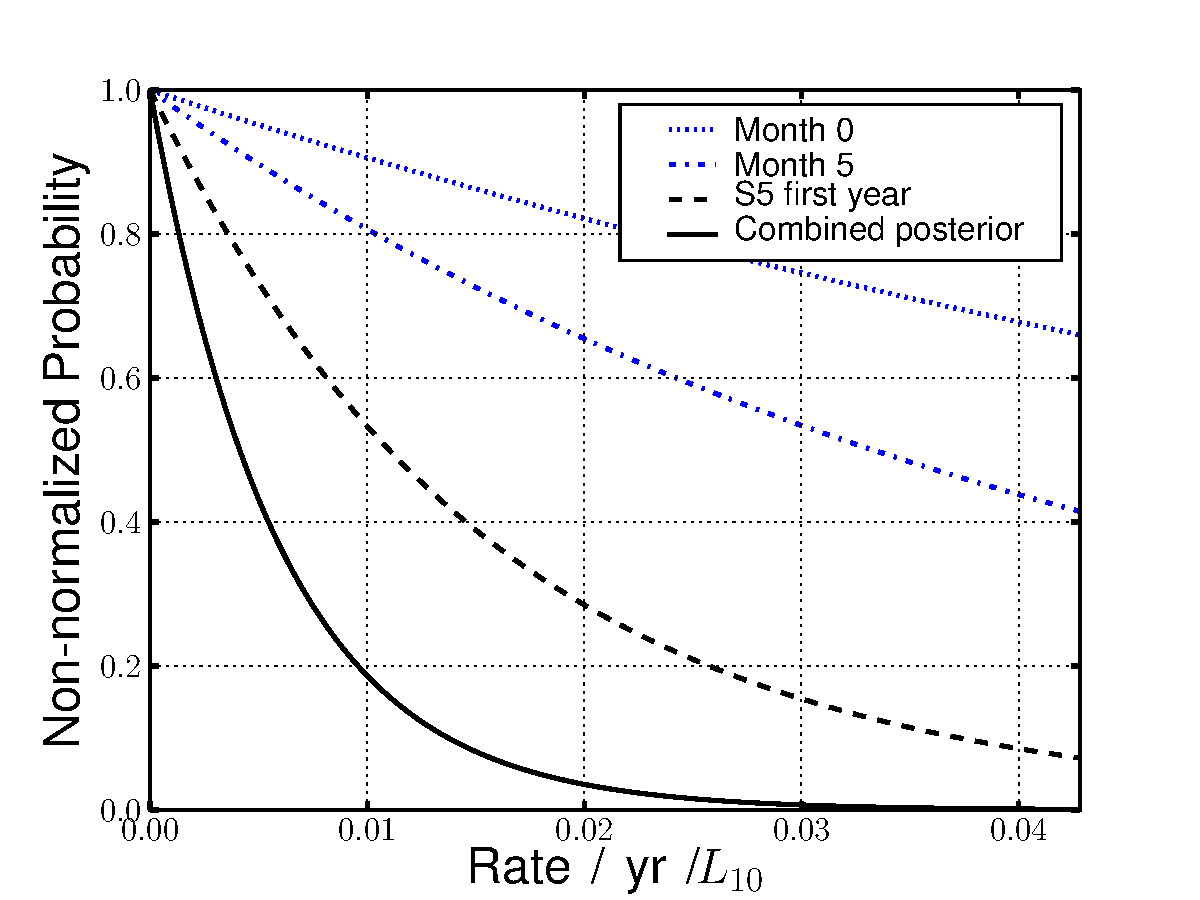
\includegraphics[width=6in]{figures/S5_lowmass_18_month_combined_bns_nonspin-posterior-comparison}
\caption{The posterior distribution for the rate of BNS coalescences. The
dashed black curve shows the rate computed in ~\cite{Collaboration:2009tt}.
The solid black curve shows the result of this search using the previous
analysis as a prior. The figure also shows the rate distributions for two of
the  individual months computed using a uniform prior. The improvement from
month 0 to month 5 is due to increasing detector sensitivity during this
search.  }  
   \label{fig:ul}
\end{figure}

The rate of instrumental noise artifacts was measured by time-shifting data
from the Livingston and Hanford observatories (H1 and H2 data are kept fixed
with respect to each other). The data was offset by more than the light-travel
time between observatories, thus triggers which survived the pipeline were due
to noise alone. We performed 100 such time-shifts to obtain a good estimate of
the noise background in our search. \ac{CBC} signals of higher-mass contain
fewer gravitational-wave cycles in the sensitive band of our detectors: our
signal-based vetoes were not as powerful. High-mass templates are therefore
more sensitive to non-stationary noise transients and hence our \ac{FAR} for
these system is larger. In order to account for this mass-dependent behavior we
computed the background for three different mass regions and compared
foreground and background within each of these ranges. Specifically, in each
region we counted the number of background triggers with effective \ac{SNR}
greater-than or equal-to a given foreground trigger; dividing this number by
the amount of background time analyzed gave us the \ac{FAR} for that trigger.
This allowed us to define a single detection statistic for every trigger in
each of the mass categories.  The \ac{FAR} could then be directly compared to
obtain a ranking of the significance of the triggers, regardless of their
mass~\cite{Collaboration:2009tt}. 

%%%%%%%%%%%%%%%%%%%%%%%%%%%%%%%%%%%%%%%
\section{Search results}
\label{sec:results}

The seven months of data were analyzed separately using the procedure described
above. No gravitational-wave candidates were observed with a \ac{FAR}
significantly above those expected from the noise background.  The loudest
trigger in this search was a triple coincident trigger with a FAR of $6$ per
year. This is consistent with the expected background, since we searched
$0.21$~yr of data. The second and third loudest triggers had FAR values of $10$
and $11$ per year, respectively. Although we did not have any detection
candidates, we exercised our follow-up procedures by examining any triggers
with a \ac{FAR} of less than $50$ per year.  This exercise prepares us for
future detections and often identifies areas where our search pipeline can be
improved to exclude noise transients.

In the absence of detection candidates, we used our observations to set an
upper limit on CBC rates. We followed the procedure described
in~\cite{Fairhurst:2007qj,loudestGWDAW03,Biswas:2007ni} and used the results
reported in ~\cite{Collaboration:2009tt} as prior information on the rates.  We
present five different classes of upper limits.  The first three limits are
placed on binaries of neutron stars and/or black holes assuming canonical mass
distributions for \ac{BNS} $[m_1 = m_2 = (1.35\pm 0.04)~\Msun]$, \ac{BBH} $[m_1
= m_2 = (5\pm 1)~\Msun]$, and \ac{NSBH} $[m_1 = (5\pm 1)~\Msun,~m_2 = (1.35\pm
0.04)~\Msun]$ systems.  We also present upper limits as a function of the total
mass of the binary and, for \ac{NSBH} binaries, as a function of the black hole
mass. We combined the results from each of the seven months, along with the
prior results from the first year analysis, in a Bayesian manner, using the
same procedure as described in~\cite{Collaboration:2009tt}.

We first calculated upper limits on \ac{BNS}, \ac{BBH} and \ac{NSBH} systems
assuming the objects have no spin; these results are summarized in Tables
\ref{tab:bns} and \ref{tab:ul}.  The rate of binary coalescences in a galaxy is
expected to be proportional to the blue light luminosity of the
galaxy~\cite{LIGOS3S4Galaxies}.  Therefore, we placed limits on the rate per
$\mathrm{L}_{10}$ per year, where $\mathrm{L}_{10}$ is $10^{10}$ times the blue
solar luminosity (the Milky Way contains $\sim 1.7
\mathrm{L}_{10}$~\cite{Kalogera:2000dz}).  To calculate the search sensitivity,
the analysis was repeated numerous times adding simulated signals with a range
of masses, distance and other astrophysical parameters to the data. Table
\ref{tab:ul} shows the sensitivity of the LIGO detectors to coalescing binaries
quoted in terms of the horizon distance, i.e., the distance at which an
optimally oriented and located binary would produce an \ac{SNR} of 8.  

There are a number of uncertainties which affected the upper limit calculation,
including Monte Carlo statistics, detector calibration, distances and
luminosities of galaxies listed in the galaxy catalog~\cite{LIGOS3S4Galaxies},
and differences between the \ac{pN} templates used to evaluate efficiency of
the search and the actual waveforms.  The effect of these errors on the
cumulative luminosity are summarized for the \ac{BNS} search in
Table~\ref{tab:bns}.  We marginalized over all of the
uncertainties~\cite{Fairhurst:2007qj} to obtain a posterior distribution on the
rate of binary coalescences.  

In Fig.~\ref{fig:ul}, we show the derived distribution of the rate of
\ac{BNS} coalescences. The distribution is peaked at zero rate
because there were no detection candidates.  We include the distribution for
all searches previous to this one (which was our prior).  In addition, we
present the result that would be obtained from each month, were it
analyzed independently of the others and of the previous searches.  This
provides an illustration of the amount that each month contributes to
the final upper limit result, and demonstrates the improvement in
sensitivity of the detectors during the search.  The upper limit is
finally obtained by integrating the distribution from zero to
$\mathcal{R}_{90\%}$ so that $90\%$ of the probability is contained in the
interval.  The results obtained in this way were:
%
%\begin{eqnarray}
$\mathcal{R}_{90\%,{\rm BNS}} = \BNSul\,
\textrm{yr}^{-1}\mathrm{L_{10}}^{-1} \, ,
\mathcal{R}_{90\%,{\rm BBH}} = \BBHul\,
\textrm{yr}^{-1}\mathrm{L_{10}}^{-1} \, , \text{ and }
\mathcal{R}_{90\%,{\rm NSBH}} =  \NSBHul\,
\textrm{yr}^{-1}\mathrm{L_{10}}^{-1} \, .$
%\end{eqnarray}


Additionally, we calculated the upper limit for BBH systems as a function of
the total mass of the binary, assuming a uniform distribution of the component
masses.  For \ac{NSBH} systems, we constructed an upper limit as a function of
the black hole mass, assuming a fixed neutron star mass of $m_{\mathrm{NS}} =
1.35 \Msun$.  These upper limits are shown in Fig~\ref{fig:ulmass}.

%\input{ulTable1}
\begin{table}[t]
\center
\begin{tabular}{c | c | c | c}
\hline \hline
\multicolumn{1}{m{5cm}|}{\centering Coincidence time} & H1H2L1 & H1L1 & H2L1 \\
\hline
\multicolumn{1}{m{5cm}|}{\centering Observation time (yr)} & 0.21 & 0.02 & 0.01 \\
\hline
\multicolumn{1}{m{5cm}|}{\centering Cumulative luminosity $\left({L_{10}}\right)$} & $\BNStripleCumLum$ & $\BNSHoneLoneCumLum$ & $\BNSHtwoLoneCumLum$ \\
\hline
\multicolumn{1}{m{5cm}|}{\centering Calibration error} & $\BNStripleCalErr$ & $\BNSHoneLoneCalErr$ & $\BNSHtwoLoneCalErr$ \\
\hline
\multicolumn{1}{m{5cm}|}{\centering Monte Carlo error} & $\BNStripleMonErr$ & $\BNSHoneLoneMonErr$ & $\BNSHtwoLoneMonErr$ \\
\hline
\multicolumn{1}{m{5cm}|}{\centering Waveform error} & $\BNStripleWavErr$ & $\BNSHoneLoneWavErr$ & $\BNSHtwoLoneWavErr$ \\
\hline
\multicolumn{1}{m{5cm}|}{\centering Galaxy distance error} & $\BNStripleGDErr$ & $\BNSHoneLoneGDErr$ & $\BNSHtwoLoneGDErr$ \\
\hline
\multicolumn{1}{m{5cm}|}{\centering Galaxy magnitude error} & $\BNStripleGMErr$ & $\BNSHoneLoneGMErr$ & $\BNSHtwoLoneGMErr$ \\
\hline
\hline
\end{tabular}
\caption{Detailed results from the BNS search.  The observation
time is the time used in the upper limit analysis.  The cumulative
luminosity is the luminosity to which the search was sensitive above the
loudest event for each coincidence time.  The errors in this table are
listed as one-sigma logarithmic error bars (expressed as percentages) in
luminosity associated with each source error.}
\label{tab:bns}
\end{table}


%\input{ulTable2}
\begin{table}[t]
\center
\begin{tabular}{c | c | c | c}
\hline \hline
\multicolumn{1}{m{3cm}|}{\centering Component masses $\left(M_{\odot}\right)$} & 1.35/1.35 & 5.0/5.0 & 5.0/1.35 \\
\hline
\multicolumn{1}{m{3cm}|}{\centering $D_{\rm horizon}$ $\left({\rm Mpc}\right)$} & $\sim 30$ & $\sim 100$ & $\sim 60$ \\
\hline
\multicolumn{1}{m{3cm}|}{\centering Cumulative lminosity $\left({L_{10}}\right)$} & 490 & 11000 & 2100 \\
\hline
\multicolumn{1}{m{3cm}|}{\centering Nonspinning upper limit $\left({{\rm yr}^{-1} L_{10}^{-1}}\right)$} & \BNSul & \BBHul & \NSBHul \\
\hline
\multicolumn{1}{m{3cm}|}{\centering Spinning upper limit $\left({{\rm yr}^{-1} L_{10}^{-1}}\right)$} & ... & \SBBHul & \SNSBHul \\
\hline
\hline
\end{tabular}
\caption{Overview of results from BNS, BBH and NSBH
searches.  $D_{\rm horizon}$ is the horizon distance 
averaged over the time of the search.  The cumulative luminosity is the
luminosity to which the search was sensitive above the loudest event for
times when all three LIGO detectors were operational.  The first
set of upper limits are those obtained for binaries with non-spinning
components.  The second set of upper limits are produced using black
holes with a spin uniformly distributed between zero and the maximal
value of $G m^{2}/c$.}
\label{tab:ul}
\end{table}


\begin{figure}[ht] 
\center
\subfigure{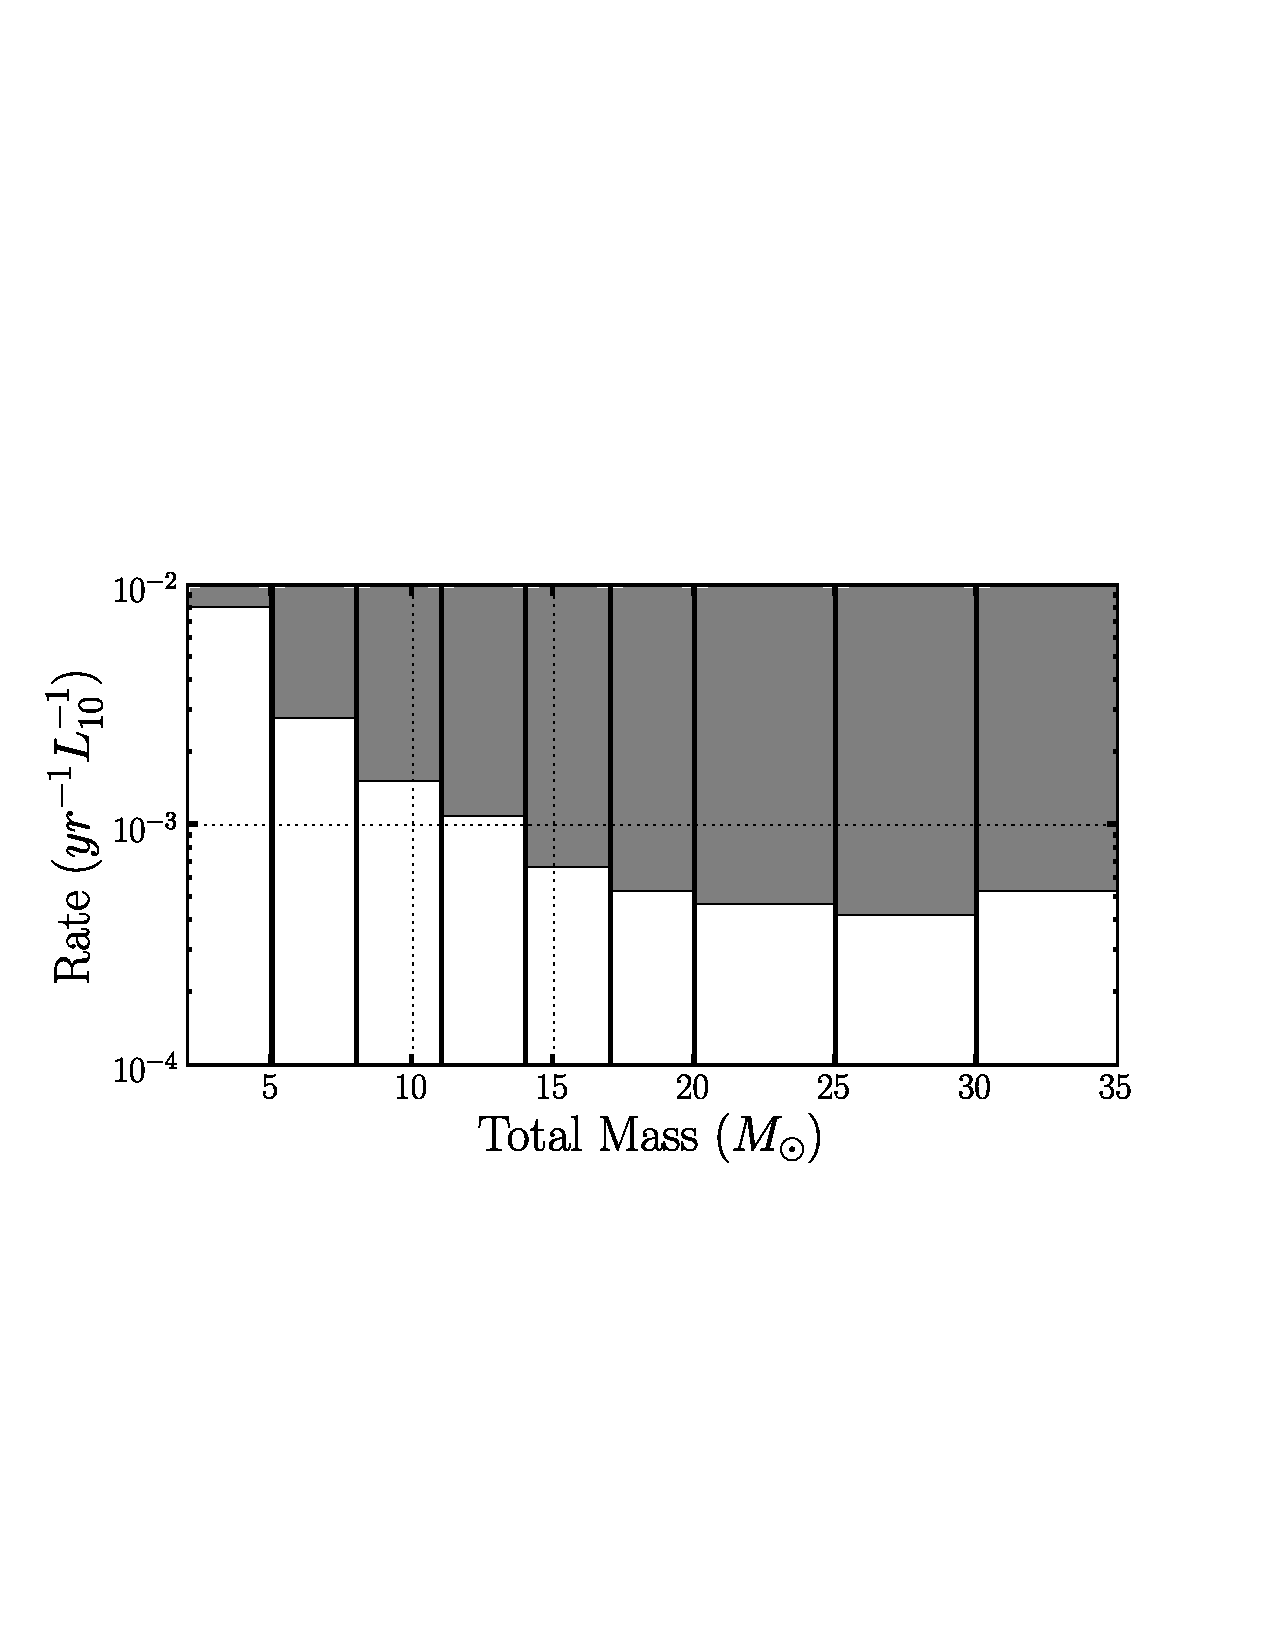
\includegraphics[width=6in]{figures/S5_lowmass_18_month_combined_mtotal_nonspin-combined-rate-v-mass}\vspace*{0.15cm}}
\subfigure{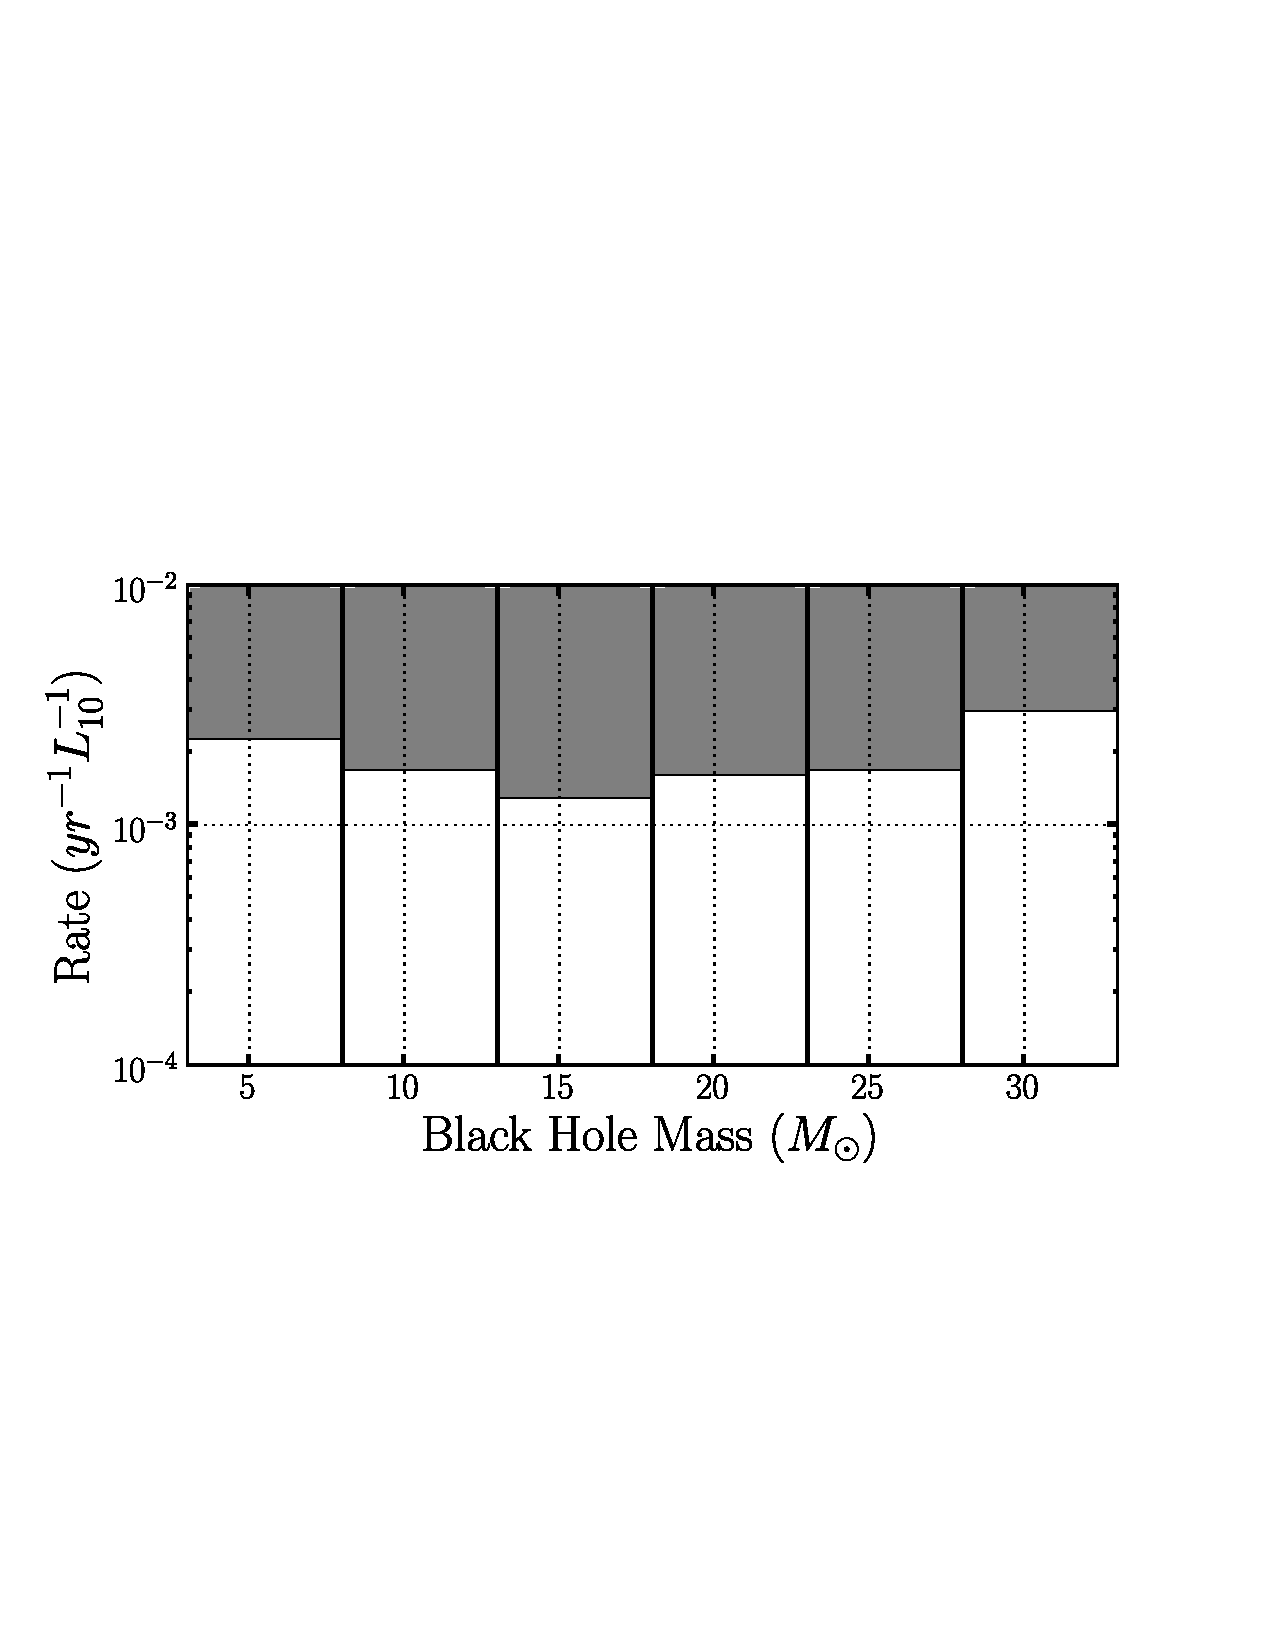
\includegraphics[width=6in]{figures/S5_lowmass_18_month_combined_mcomp_nonspin-combined-rate-v-mass}}
  \caption{The marginalized 90\% rate upper limits as a function of mass.  The
upper plot shows limits for BBH systems as a function of the
total mass of the system.  The lower plot shows limits for NSBH
systems as a function of the black hole mass, assuming a fixed
neutron star mass of $1.35 M_{\odot}$. Here the upper limits were 
calculated using only H1H2L1 data since the relatively small amount
of H1L1 and H2L1 data made it difficult to 
evaluate the cumulative luminosity in the individual mass bins.} 
  \label{fig:ulmass}
\end{figure}
Finally, we present upper limits on coalescence rates where the spin of
the components of the binary is taken into account.  Astrophysical
observations of neutron stars indicate that their spins will not be
large enough to have a significant effect on the BNS waveform
observed in the LIGO band~\cite{ATNF:psrcat,Apostolatos:1994}.
Theoretical considerations limit the magnitude of the spin, $S$, of a
black hole to lie within the range $0 \le S \le G m^{2}/c$.  However,
the astrophysical distribution of black hole spins, and spin
orientations, is not well constrained.  Therefore, we provide a sample
upper limit for spinning systems using a spin magnitude and orientation
distributed uniformly within the allowed values.  This gives upper
limits on the rate of BBH and NSBH systems of:
%
%\begin{eqnarray}
$\mathcal{R}_{90\%,{\rm BBH}} = \SBBHul\,
\textrm{ yr}^{-1}\mathrm{L_{10}}^{-1} \text{ and }
\mathcal{R}_{90\%,{\rm NSBH}} =  \SNSBHul\,
\textrm{ yr}^{-1}\mathrm{L_{10}}^{-1} \, .$
%\end{eqnarray}
%
These rates are about $20\%$ larger than the non-spinning rates.

\paragraph{Discussion}

We searched for gravitational waves from CBCs with total mass between $2$ and
$35\, M_\odot$ in \ac{LIGO} observations between November 14, 2006 and May 18,
2007.  No detection candidates with significance above that expected due to
background were found in the search. By combining this search with our previous
results, we set a new upper limit on the CBC rate in the local universe which
is approximately a factor of $3$ lower than that reported in
~\cite{Collaboration:2009tt}.  This improvement was significant, even though we
searched only two thirds as much data as in ~\cite{Collaboration:2009tt}.  It
was due, in part, to improvements in detector sensitivity during the second
year of S5 which increased the horizon distance.  Moreover, the shorter
analysis time and improved stationarity of the data led to many of the months
having a less-significant loudest event than in the previous search.  Both of
these effects increased the luminosity to which the search was sensitive,
thereby improving the upper limit.

Astrophysical estimates for \ac{CBC} rates depend on a number of assumptions
and unknown model parameters, and are still uncertain at present.  In the
simplest models, the coalescence rates should be proportional to the stellar
birth rate in nearby spiral galaxies, which can be estimated from their
blue-light luminosity \cite{LIGOS3S4Galaxies}.  The optimistic, upper end of
the plausible rate range for \ac{BNS} is $5 \times 10^{-4} \textrm{ yr}^{-1}
\mathrm{L}_{10}^{-1}$~\cite{Kalogera:2004tn, Kalogera:2004nt} and $6 \times
10^{-5} \textrm{ yr}^{-1} \mathrm{L}_{10}^{-1}$ for \ac{BBH} and \ac{NSBH}
\cite{Oshaughnessy:2008, OShaughnessy:2005}.  The upper limits reported here
are $\sim 1$--$2$ orders of magnitude above the optimistic expected rates.  The
most confident \ac{BNS} rate predictions are based on extrapolations from
observed binary pulsars in our Galaxy; these yield realistic \ac{BNS} rates of
$5 \times 10^{-5} \textrm{ yr}^{-1}
\mathrm{L}_{10}^{-1}$~\cite{Kalogera:2004tn, Kalogera:2004nt}.  Rate estimates
for \ac{BBH} and \ac{NSBH} are less well constrained, but realistic estimates
are $2 \times 10^{-6} \textrm{ yr}^{-1} \mathrm{L}_{10}^{-1}$ for \ac{NSBH}
\cite{Oshaughnessy:2008} and $4 \times 10^{-7} \textrm{ yr}^{-1}
\mathrm{L}_{10}^{-1}$ for \ac{BBH} \cite{OShaughnessy:2005}.  Thus, the
expected rates are $\sim 2$--$3$ orders of magnitude lower than the limits
presented in this chapter. The Advanced LIGO and Virgo detectors, currently
under construction, will increase our horizon distance by an order of magnitude
or more, allowing us to measure the rate of CBCs in the Universe.
